\documentclass{exam}
\usepackage[utf8]{inputenc}
\usepackage{pgfplots}
\title{PHYS 231 Harmonic Motion}
\author{Collin McDevitt }
\date{November 2022}

\begin{document}

\maketitle


\large

\begin{questions}
\question What is the spring constant of a spring that starts 10.0 cm long and extends to 11.4 cm with a 300 g mass hanging from it? 
\vspace{10mm}
\question List three places besides in springs where Hooke's law applies.
\vspace{10mm}
\question Show that $x(t)= A\cos(\omega t)+ B\sin(\omega t) $is a solution to the differential equation of the mass/spring system.
\vspace{20mm}
\question  Does the period of simple harmonic motion depend on amplitude?  
\vspace{20mm}
\question  On what does the period of a mass on a spring depend?
\vspace{10mm}
 \question  Is the true pendulum an example of SHM?  Explain.
\vspace{15mm}
\question 
What is the point of using a Taylor series in the context of the pendulum differential equation?
\vspace{15mm}
\question What period do you expect to find for small amplitude swinging motion of a rock tied to a 1.0 m long string?
\vspace{15mm}
\question
Using the animated slider in the book, estimate the period of the same rock caused to swing at a 90 degree angle from vertical.  NOTE: It is possible to drag and zoom the plot in the book to get a precise answer.
\vspace{15mm}
\question
Why does the actual pendulum's plot of angle vs time flatten out at very large swing angles?  Give a clear physical explanation.
\vspace{15mm}
\question At what point in SHM is the velocity maximum?  Displacement maximum?
\vspace{15mm}
\question{}
What could we conclude if a system has a phase trajectory that sweeps out larger and larger area as time goes by?
\vspace{15mm}
\question
What does a repetitive phase trajectory indicate about a system?
\vspace{15mm}
\question
What does each point in phase space represent?
\vspace{15mm}
\question Given an oscillator of mass 2.0kg and spring constant of 180N/m, what is the period without damping?  Use numerical methods to model this oscillator with an additional friction force equal to $F_{dampaning} = -cv$ where c is a positive damping constant.  Using c=5.0, what is the new period of oscillation.  What about for c=10? Assume initial position is 0.2m and initial velocity is zero.  Please find the period using the position versus time plot and use the first full cycle of the motion.
\begin{center}
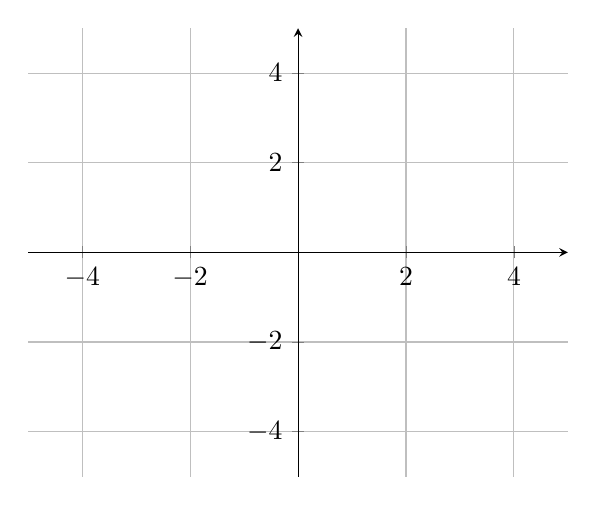
\begin{tikzpicture}
\vspace{5mm}

    

\begin{axis}[xmin=-5, xmax=5, ymin=-5, ymax=5, axis x line=middle, axis y line=middle,grid = both]

\end{axis}
\end{tikzpicture}
\end{center}
\vspace{15mm}
\question Critical damping is the case where the mass never actually crosses over equilibrium position, but reaches equilibrium as fast as possible.  Experiment with changing c to find the critical damping constant.  Use the same initial conditions as in the last problem.  Zoom in a bit to make sure you don't allow any oscillations to take place - even small ones.
\vspace{40mm}
\question 
 Shocks on cars are usually designed to achieve critical damping of the suspension system when the car is loaded with maximum number of passengers and cargo.  With only a driver and minimum cargo, is the car over-damped or under-damped?  Over-damped means even more damping than the critical amount and under means the opposite.
\vspace{60mm}
\question
A 2.0kg mass on a spring with elastic constant 32 N/m starts at a position of x=0.3m away from equilibrium with a velocity of 0.4 m/s.  What will its maximum displacement be?  Maximum velocity?  Maximum acceleration?  What will those three values be at t=5.0s?
\vspace{60mm}
\question
A pendulum length is doubled.  What happens to its period?
\vspace{15mm}
\question
A mass hanging from a pendulum is doubled.  What happens to the period?
 

\end{questions}


\end{document}
